\documentclass[UTF8]{ctexart}
\usepackage{subfiles}  

%下面的语句, 引入你的头部设置文件
\usepackage{C:/phpStorm_proj/02_myself_ID_EGO/+100_latex_all_math_sel/myPreamble} 
%必须是绝对路径,才能让各个tex在单独编译时使用到

\title{向量组的线性相关性}


%---------------------------------


\begin{document}
\tableofcontents % 生成目录
\date{} % 若不写这句, 则默认也会渲染出日期, 所以我们要手动赋空值
\maketitle  %这行代码, 让你前面的 title, author, date生效

\section{向量 vector 的几何意义}

\subsection{向量, 就是箭头线段的``终点"坐标}

通常, 当你考虑``一个"向量时, 就把它看成是``箭头". \\
当你考虑``多个"向量时, 就把它看成是``箭头终点"的那个点(point).\\

\textbf{注意: 向量的值, 表示的是坐标轴的位置, 而不是该向量线段的长度(即不是`模"的概念).}\\

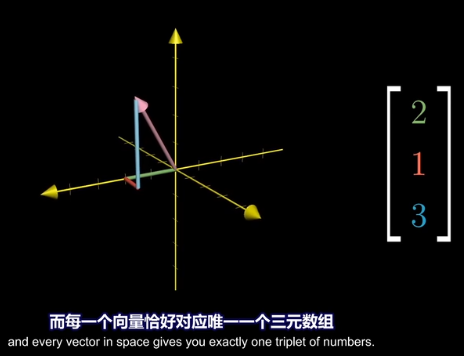
\includegraphics[width=0.4\textwidth]{img/0066.png}\\




~\\
\hrule
~\\

\subsection{向量的``数乘" : 系数k的作用, 是把向量伸缩 k倍}

$2\left| \begin{array}{l}
		x \\
		y \\
	\end{array} \right|=\left| \begin{array}{l}
		2x \\
		2y \\
	\end{array} \right|
$\\

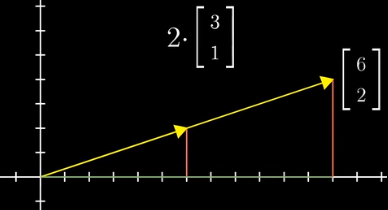
\includegraphics[width=0.4\textwidth]{img/0067.png}\\
\\


$text{其充要条件是:\ 要么\ 数}k=0,\ \text{或要么\ }\alpha =0\text{向量}$


~\\
\hrule
~\\


\subsection{单位向量 : 基 basis}

The \textbf{basis} of a vector space /is a set of linearly independent vectors /that span the full space.

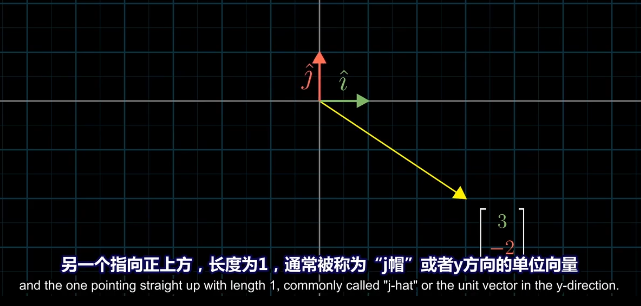
\includegraphics[width=0.6\textwidth]{img/0068.png}\\

$\left. \begin{array}{r}
		\hat{i} = 1 \\
		\hat{j} = 1 \\
	\end{array} \right\}$ ← 称为``单位向量"或``基"\\

事实上, 每当我们描述一个向量时, 它都依赖于我们正在使用的``基".\\

$\vec{v}=\left| \begin{array}{l}
		3  \\
		-2 \\
	\end{array} \right|= 3 \hat{i} + (-2)\hat{j}$\\

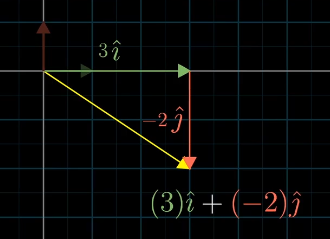
\includegraphics[width=0.3\textwidth]{img/0069.png}\\

向量的终点坐标, 其实就是系数倍的``基向量"的线性组合.\\



【你可以选择任意两个方向作为``基", 只要它们互相垂直即可.】 \\
比如,你可以选择指向右上方的向量 v, 和 指向右下方的向量 w, 作为基向量. \\
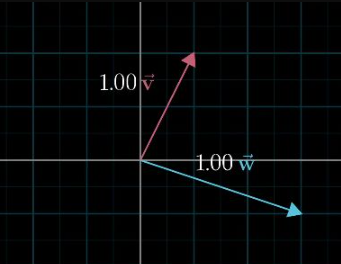
\includegraphics[width=0.35\textwidth]{img/0102.png}\\

这组新的基向量, 进行缩放, 再相加,同样能构造出其他的向量.\\
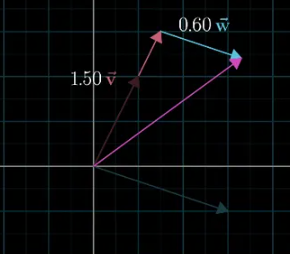
\includegraphics[width=0.35\textwidth]{img/0103.png}\\

所以, 一组``基向量", 就对应一个坐标系. 选择不同的基向量, 就构造出了不同的坐标系. 同一个向量,在不同的坐标系下(即采用不同的基向量),其坐标值也要相应地发生变化. \\

上面, 反复出现\textbf{``将向量进行缩放,再相加"的操作, 这样的操作,我们称之为``线性组合".}


~\\
\hrule
~\\

\subsection{张成 span}


在二维平面中,选取 2 个向量, ,然后考虑它们所有可能的``线性组合", 我们会得到什么呢? 这取决于我们选择的 2 个向量.\\

→ 通常情况下,我们会得到整个平面.\\
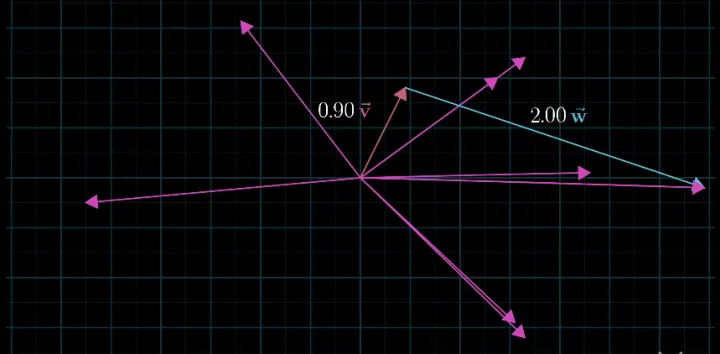
\includegraphics[width=0.7\textwidth]{img/0104.png}\\

→ 但如果选择的 2 个向量,恰好``共线"的话,那它们的线性组合, 就被局限在一条过原点的直线上了. \\
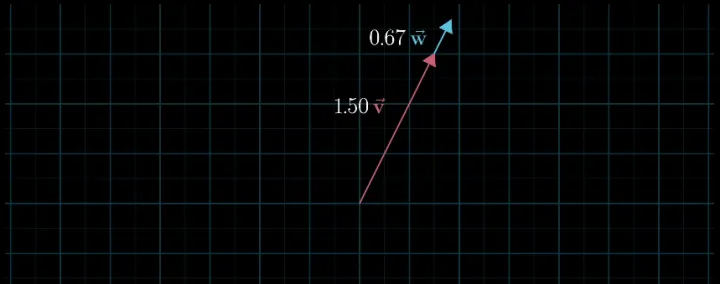
\includegraphics[width=0.7\textwidth]{img/0105.png}\\

→ 最极端的情况是,如果选择的 2 个向量都是零向量,那么它们的线性组合, 就只可能是零向量了. \\
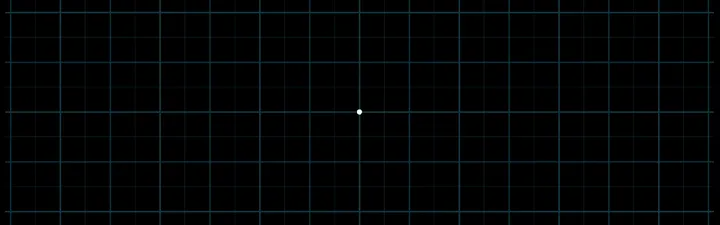
\includegraphics[width=0.7\textwidth]{img/0106.png}\\

``数乘"和``加法", 是向量的两个最基础的运算. \textbf{当我们谈论向量所``张成"的空间时,我们实际上就是在问: 仅仅通过``数乘"和``加法''这两种运算,你能获得的所有可能的向量集合是什么.} \\

在线性代数中,向量的起点, 始终固定在``原点"的位置,因此, 向量的终点就唯一确定了向量本身. 这样,我们便可以将向量, 看成是``空间中的点"(即``向量的终点").\\


the span of $\vec{v}$ and $\vec{w} $  /is the set of  all their linear combinations.\\
the set of all possible vectors /than you can reach /is called the span of those two vectors. ← 相当于``势力范围", 就是张成.\\


两个斜率不同的向量(a,b), 自由伸缩, 它们的和(即a+b=c), 即新向量c的终点, 能遍及二维平面上的任何点处.\\

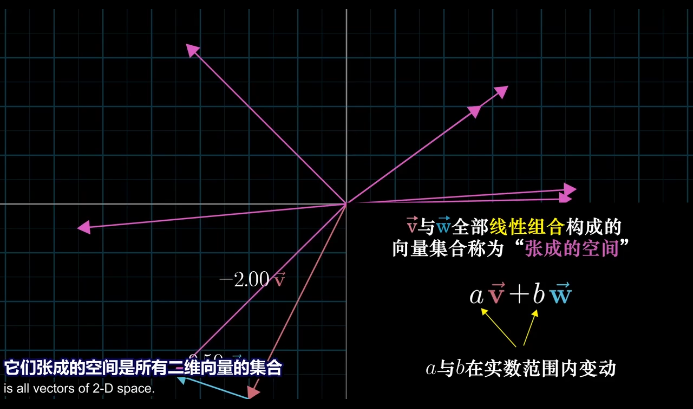
\includegraphics[width=0.6\textwidth]{img/0070.png}\\

但如果两个向量都是``零向量"的话, 它们的系数倍的和, 也永远被束缚在原点(0,0)了. $ k_1 \vec{0}  +  k_2 \vec{0}=0$ \\

三维空间中, 两个斜率同的向量, 能``张成"出``过原点"的一个平面.\\
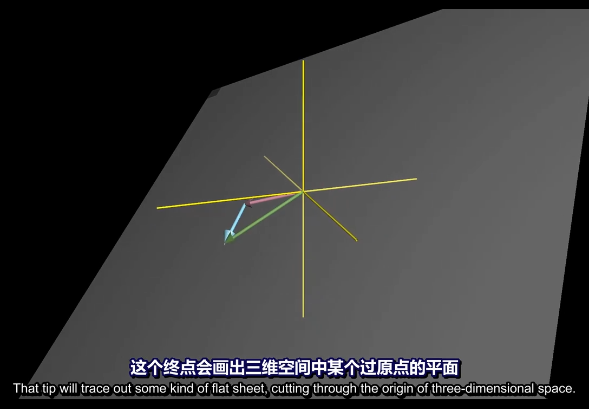
\includegraphics[width=0.4\textwidth]{img/0071.png}\\

三维空间中, 三个斜率不同的向量, 它们的和, 能张成出三维空间中所有的地方. \\
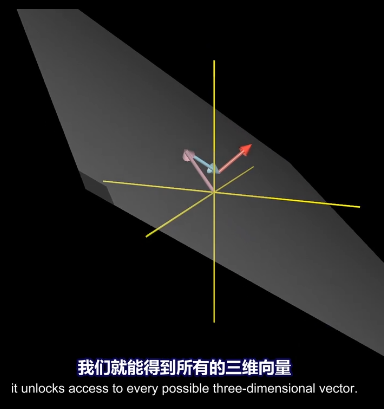
\includegraphics[width=0.4\textwidth]{img/0072.png}\\


~\\
\hrule
~\\

\section{向量的叉积(外积) : $\vec{v} \times \vec{w}$}

向量的 叉积 (外积) exterior product 或  cross product



\subsection{叉积(外积) 的几何意义 : (1)在二维空间中, 是由这两个向量围成的``平行四边形"的面积, 即是一个数值. (2)在三维空间中, 是一个垂直于这个``平行四边形"平面的``新向量".}

【在二维空间中】: \\

\textbf{几何意义上, 叉积, $\vec{v} \times \vec{w}$, 就是由这两个向量围成的``平行四边形"的面积.} \\
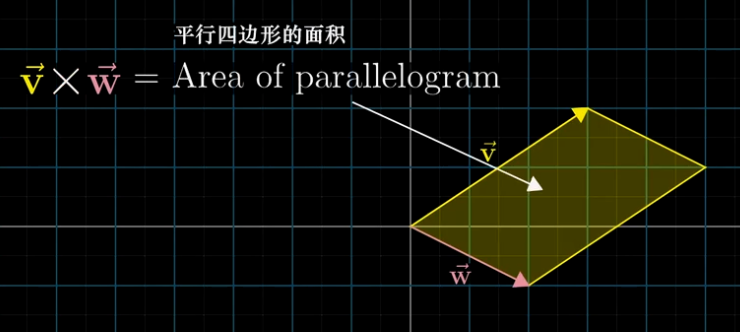
\includegraphics[width=0.5\textwidth]{img/0073.png}\\

\textbf{注意: 顺序会对``叉积"有影响: 如果$\vec{v} \times \vec{w}$ 是正数, 则 $\vec{w} \times \vec{v}$ 就是负数. 即: 交换叉乘时的顺序, 值要变号.} \\

之前说过, 行列式的值, 就是表示的是: 将基 $i \times j$ 的面积, 缩放多少倍.\\
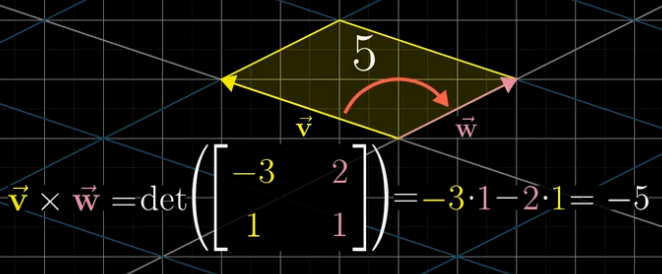
\includegraphics[width=0.5\textwidth]{img/0074.png}\\

面积的概念, 也就证明了: $3(\vec{v} \times \vec{w}) = 3 \vec{v} \times \vec{w}$\\
把平行四边形其中的任一一条边, 延长3倍 , 变成 $3 \vec{v}$ 或  $3 \vec{w}$, 面积也就是 $= 3 (\vec{v} \times \vec{w})$ \\
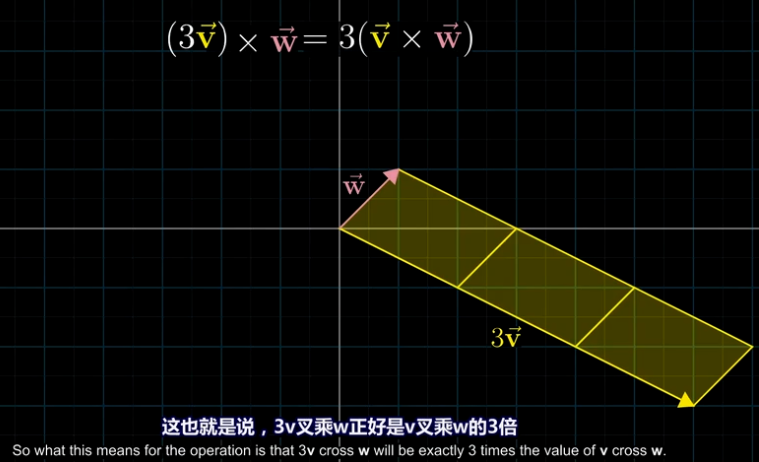
\includegraphics[width=0.5\textwidth]{img/0075.png}\\




【在三维空间中】:\\
其实, 真正的``叉积", 是通过两个三维向量, 来生成一个新的三维向量. \textbf{注意: 在三维空间中, 叉积的结果不是一个数, 而是一个向量!} \\

\begin{myEnvSample}
	如下面的图中所示, A,B两个箭头的向量的``叉积", 就是第三个向量C. 这个C向量, 始终与两个原点箭头(即A,B)正好为90度.  C向量箭头的长度, 就表示A,B向量的叉积, 它总是完全等于A,B所构成的平行四边形的面积.\\

	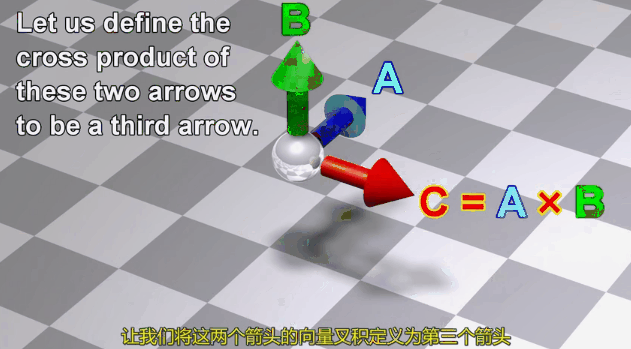
\includegraphics[width=0.4\textwidth]{img/0076.png}
	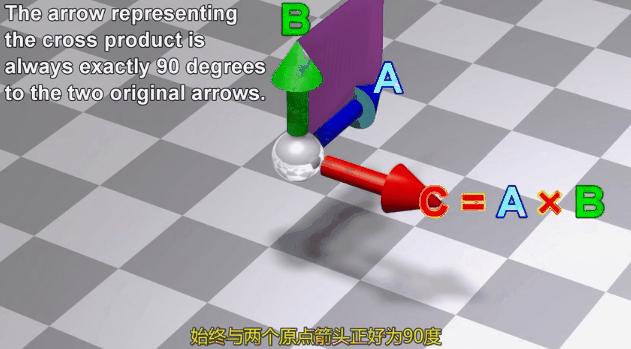
\includegraphics[width=0.4\textwidth]{img/0077.png}\\
	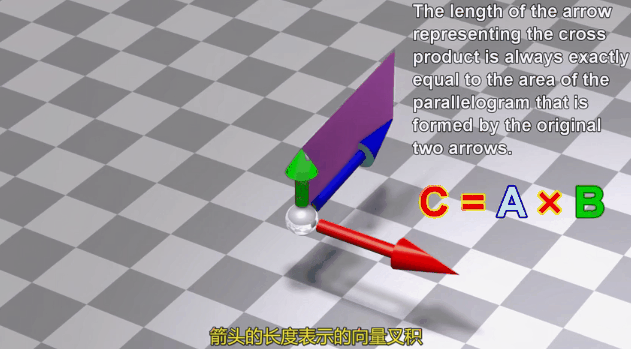
\includegraphics[width=0.4\textwidth]{img/0078.png}
	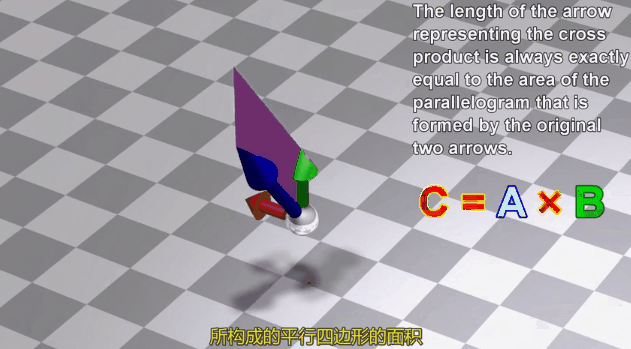
\includegraphics[width=0.4\textwidth]{img/0079.png}\\
\end{myEnvSample}


\begin{myEnvSample}
	又如: 假设$\vec{v} \times \vec{w} = 2.5$, 在三维空间中, 这两个向量构成一个平面(平行四边形). 它们的``叉积"构成一个新向量 $\vec{p}=2.5$, 它与``平行四边形"所在的面``垂直".\\

	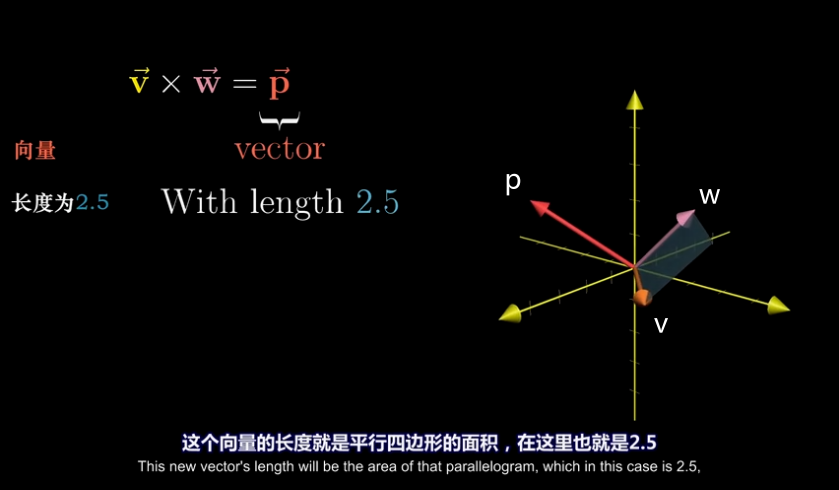
\includegraphics[width=0.7\textwidth]{img/0080.png}\\

	即: \textbf{三维叉积, 得到一个三维矢量.}   \\
	\textbf{$\vec{v} \times \vec{w}$得到新的向量$\vec{p}$,新向量$\vec{p}$的长度, 等于向$量\vec{v}$与向量$\vec{w}$组成的平行四边形的面积,并且 向量$\vec{p}$,  与 向量$\vec{v}$ 和向量$\vec{w}$所在平面垂直.}\\
	所以``三维叉积"很容易拿来算平面的``法向量". \\

	但垂直于一个平面的向量, 可以有正反两个方向, $\vec{p} $到底是朝哪个方向呢? 这就要用到"右手螺旋法则".\\

	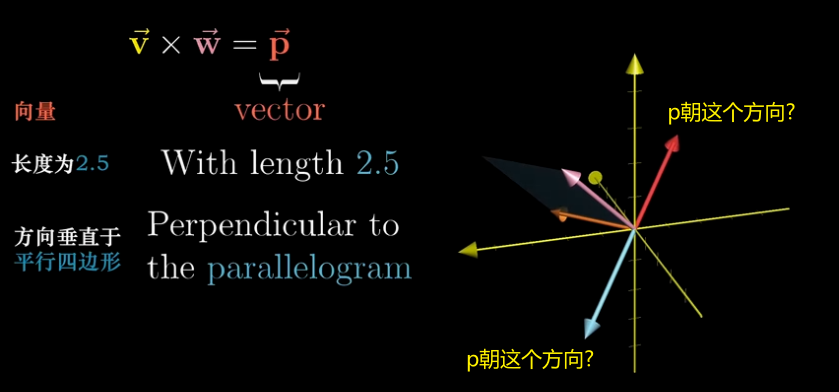
\includegraphics[width=0.7\textwidth]{img/0081.png}
\end{myEnvSample}


~\\
\hrule
~\\

\subsection{右手螺旋法则}

注意顺序: $\vec{a} \times \vec{b} = \vec{c}$, 和 $\vec{b} \times \vec{a} = \vec{c}$, ← $\vec{c}$ 的方向朝向是不同的.

\subsubsection{$\vec{a} \times \vec{b} = \vec{c}$}

1.用右手, 伸展手指, 朝向  $\vec{a}$ \\
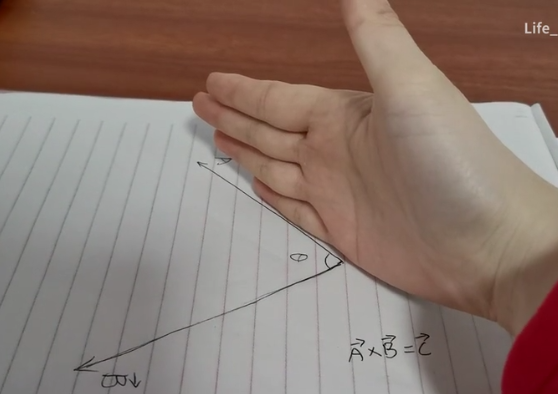
\includegraphics[width=0.3\textwidth]{img/0082.png}\\

2.然后, 握拳, 手指收回, 朝向  $\vec{b}$ 的方向. \\
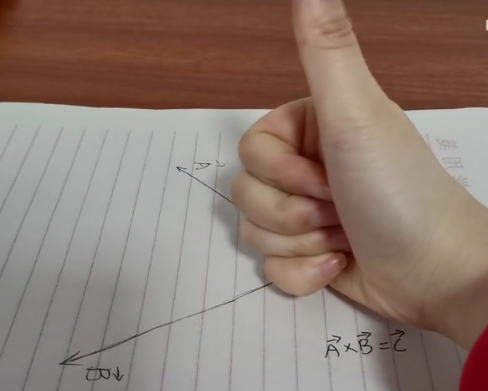
\includegraphics[width=0.3\textwidth]{img/0083.png}\\

3.则, 大拇指朝向的方向, 就是 $\vec{a} \times \vec{b} = \vec{c}$ 中, $\vec{c}$ 的朝向. \\
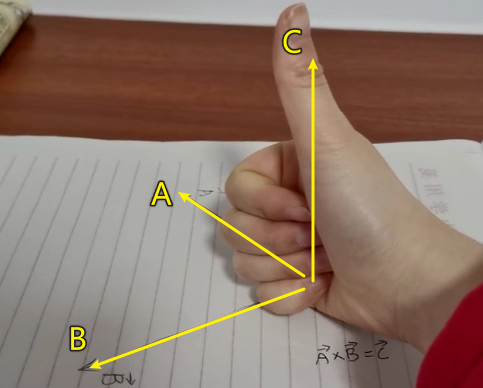
\includegraphics[width=0.3\textwidth]{img/0084.png}
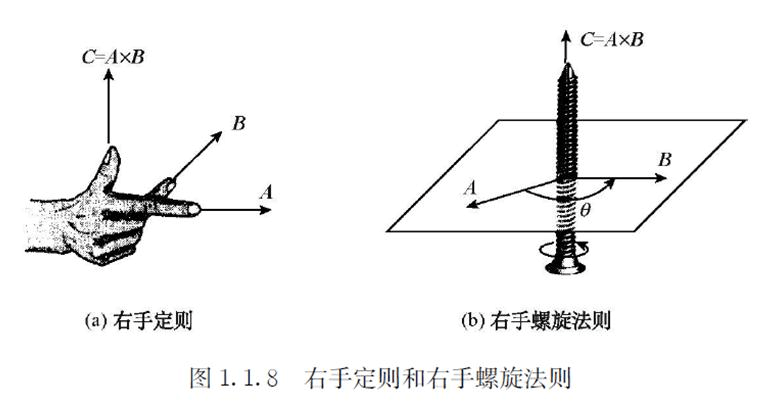
\includegraphics[width=0.65\textwidth]{img/0089.jpg}\\


\subsubsection{$\vec{b} \times \vec{a} = \vec{c}$}


1.食指朝$向\vec{b}$ 的方向. \\
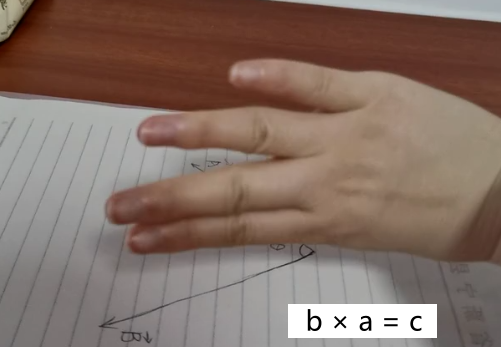
\includegraphics[width=0.3\textwidth]{img/0085.png}\\

2.握拳, 食指等收回. 此时大拇指的方向, 就是 $\vec{b} \times \vec{a} = \vec{c}$ 中 $\vec{c}$ 的朝向. \\
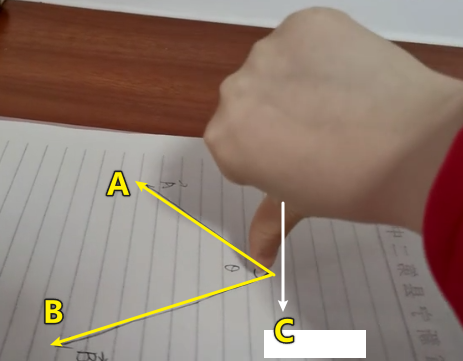
\includegraphics[width=0.3\textwidth]{img/0086.png}
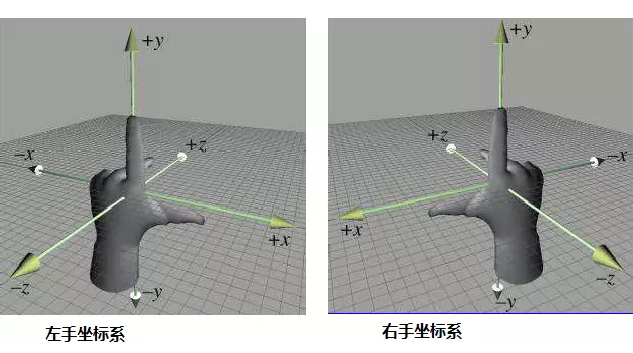
\includegraphics[width=0.65\textwidth]{img/0090.png}\\

所以, 在3D图像学中,叉乘的概念非常有用,可以通过两个向量的``叉乘",生成第三个垂直于a,b的``法向量",从而构建X、Y、Z坐标系. \\

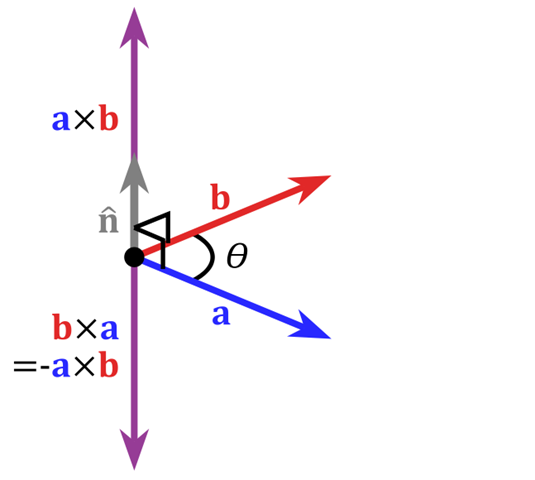
\includegraphics[width=0.3\textwidth]{img/0087.png}
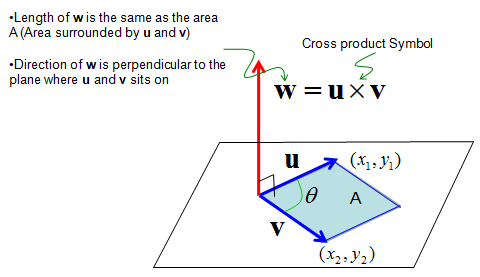
\includegraphics[width=0.5\textwidth]{img/0088.png}\\


~\\
\hrule
~\\


\section{向量的点积 (内积) : $x \cdot y = x_{1} y_{1} + x_{2} y_{2} + ...$}

\subsection{点积的几何意义: $\vec{v} \cdot \vec{w} = \vec{v} \cdot \vec{w'}$ ← 其中,$\vec{w'}$ 是 $\vec{w}$ 在 $\vec{v}$ 上的投影长度. }

→ 如果 $\vec{w'}$ 是$\vec{w}$ 在 $\vec{v}$ 上的投影长度.\\
则:  $\vec{v} \cdot \vec{w} = \vec{v} \cdot \vec{w'}$\\
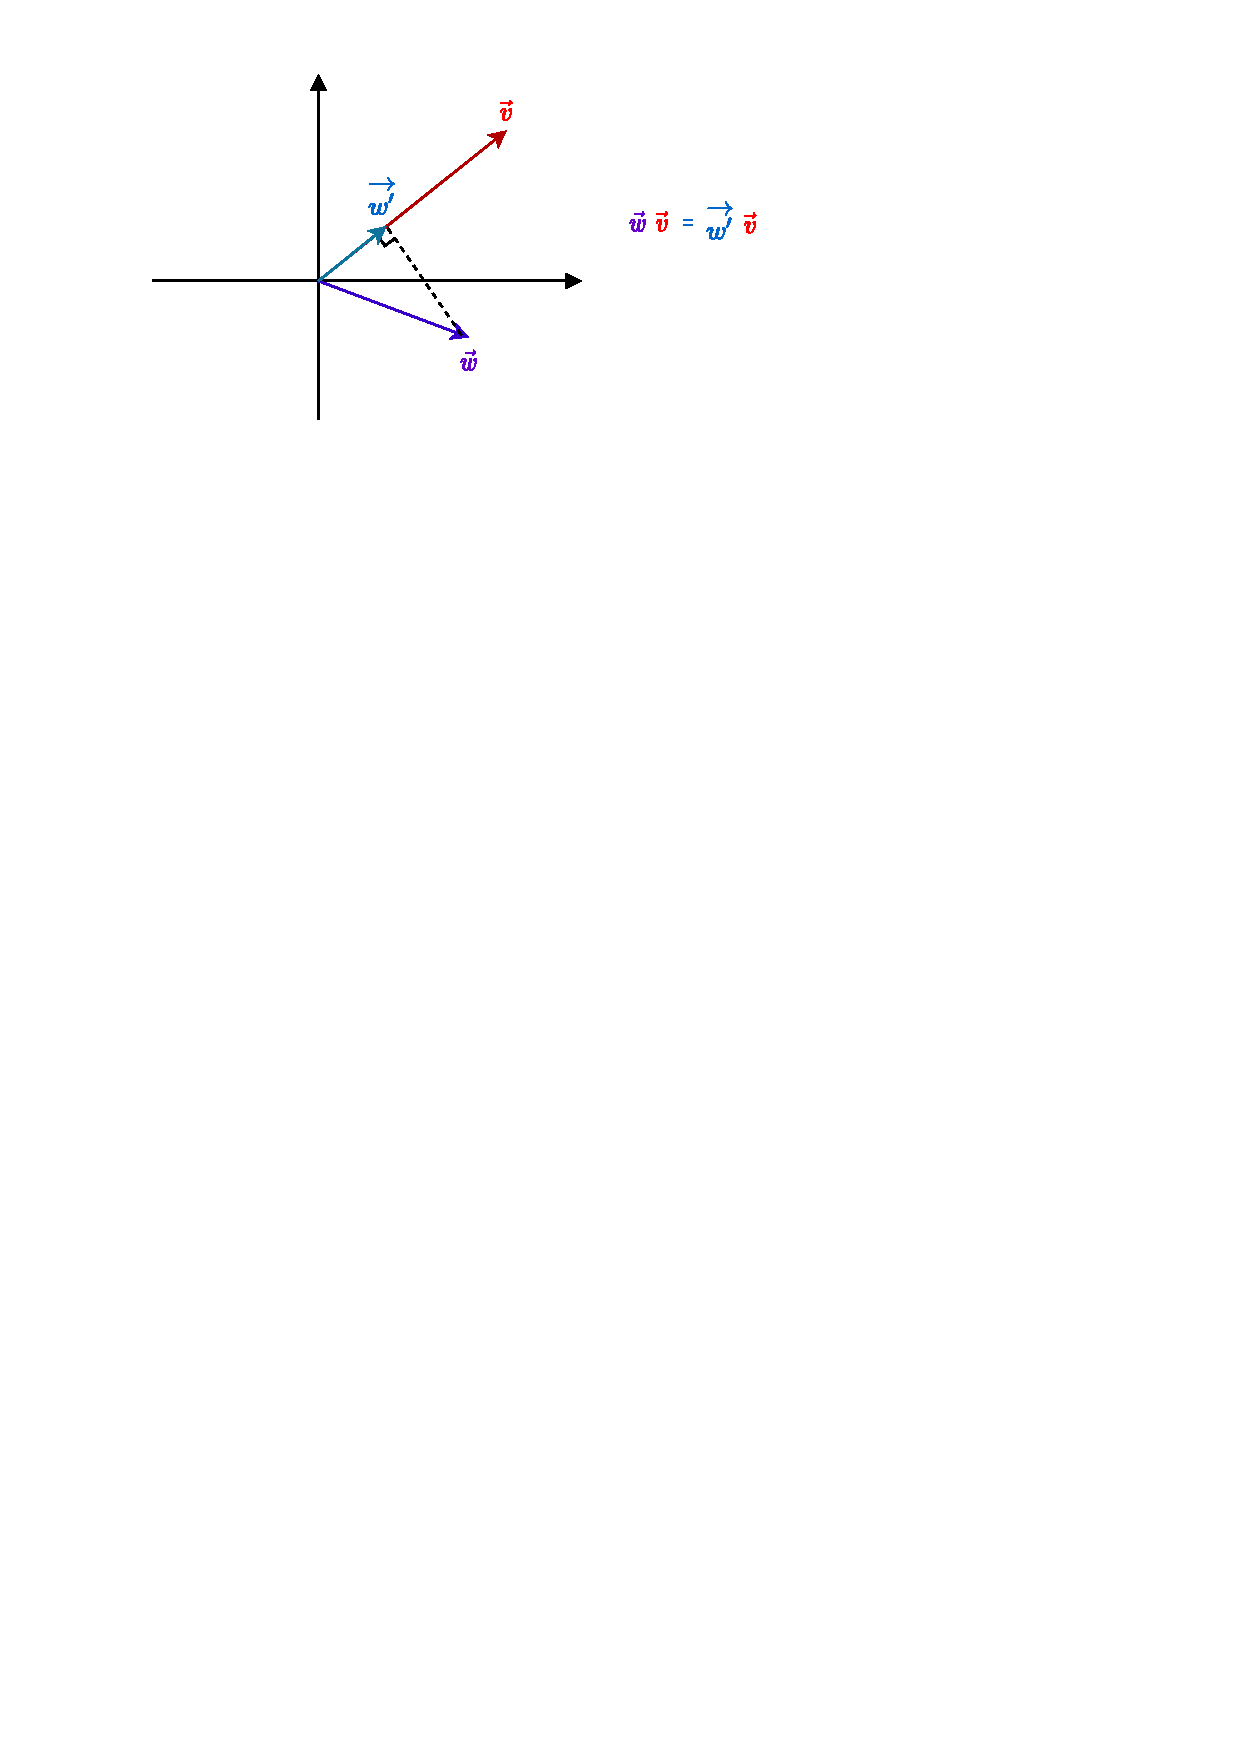
\includegraphics[width=0.4\textwidth]{img/0091.pdf}\\


→ 如果 $\vec{w}$ 的投影, 是在$\vec{v}$ 的反方向延长线上, 则此时:\\
$\vec{v} \cdot \vec{w} = \vec{v} \cdot \vec{w'} = \text{是负值}$\\
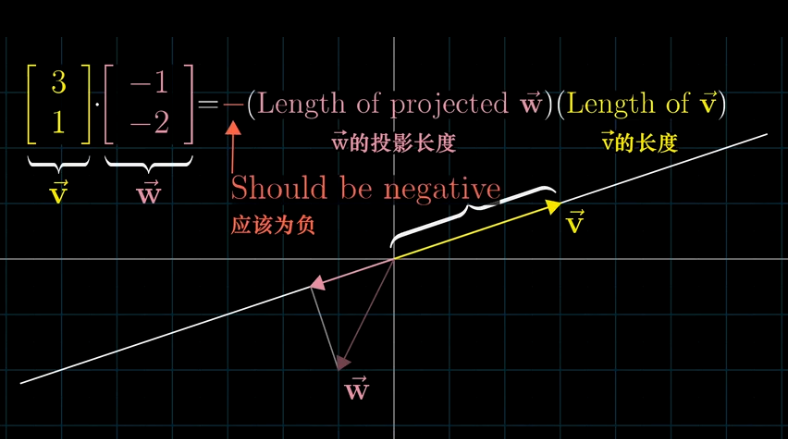
\includegraphics[width=0.6\textwidth]{img/0092.png}\\

→ 如果这两个向量, 本身就互相垂直, 则一个向量在另一个向量上的投影长度, 就为0. 这时它们的``点积"就等于0.\\
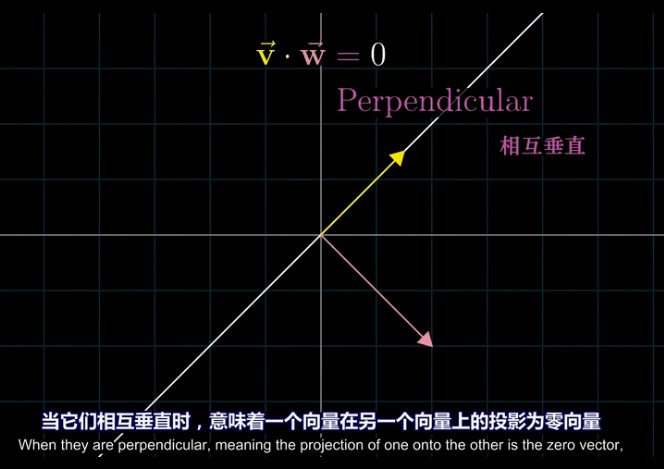
\includegraphics[width=0.5\textwidth]{img/0093.png}\\



\textbf{所以, 注意: ``点积"(inner product)运算的结果, 是一个``数"(投影的长度, 就是一个数呀). 这和向量的其他操作是有区别的.} 比如:  \\
→ 两个向量做``加法", 结果依然是个``向量". \\
→ 向量的``数乘", 结果也依然是个``向量".\\

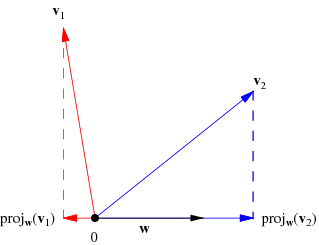
\includegraphics[width=0.4\textwidth]{img/0094.png} \\


\begin{tabular}{|l|l|}
	\hline
	若两个向量 $\vec{x}, \vec{y} $间的夹角 < 90° & $\vec{x} \cdot \vec{y} > 0$              \\
	\hline
	若 $\vec{x}, \vec{y}$ 间的夹角 > 90°         & $\vec{x} \cdot \vec{y} < 0$, 即是个负值. \\
	\hline
	若 $\vec{x}, \vec{y}$ 间的夹角 = 90°         & $\vec{x} \cdot \vec{y} = 0$              \\
	\hline
\end{tabular}





~\\
\hrule
~\\

\subsection{点积的做法公式1 : $ x\cdot y = x_1 y_{1} + x_2 y_{2} + x_{3}y_{3}$}

两个向量的"点积" (inner product  或 dot product 或 scalar product) : $\vec{x} \cdot \vec{y}$, 也有写作 <x,y> 的形式.

点积的做法公式就是:
\begin{align*}
	 & x=\left| \begin{array}{l}
		            x_1 \\
		            x_2 \\
		            x_3 \\
	            \end{array} \right|,\ y=\left| \begin{array}{l}
		                                           y_1 \\
		                                           y_2 \\
		                                           y_3 \\
	                                           \end{array} \right|, \\
	 & \text{则} :
	\boxed{
	\ x\cdot y = x_1 y_{1} + x_2 y_{2} + x_{3}y_{3}
	}
\end{align*}


即:   $x\cdot y = x^T \cdot y$  ← 即把$\vec{x}$横过来, 变成一行, 再和 $\vec{y}$ 的一列相乘. 规则和矩阵的乘法完全一样.\\
其实:   $x\cdot y = x^T \cdot y = y^T  \cdot x$\\

~\\
\hrule
~\\


\subsection{点积的做法公式2: $x \cdot y = \text{x的模} \cdot \text{y的模} \cdot cos \theta$}

两个向量的点积 = 每个向量``模长"的乘积, 再乘以它们的夹角的cos值. \\
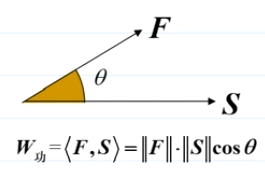
\includegraphics[width=0.25\textwidth]{img/0095.png}\\

根据"余弦定理", 有 : $a^2 = b^2 + c^2 - 2(bc \cdot \cos A) $\\
或: $\cos A = \frac{b^2 + c^2 - a^2} {2bc}$\\

那么对于由两个向量组成的三角形, 如下图, 就有: \\
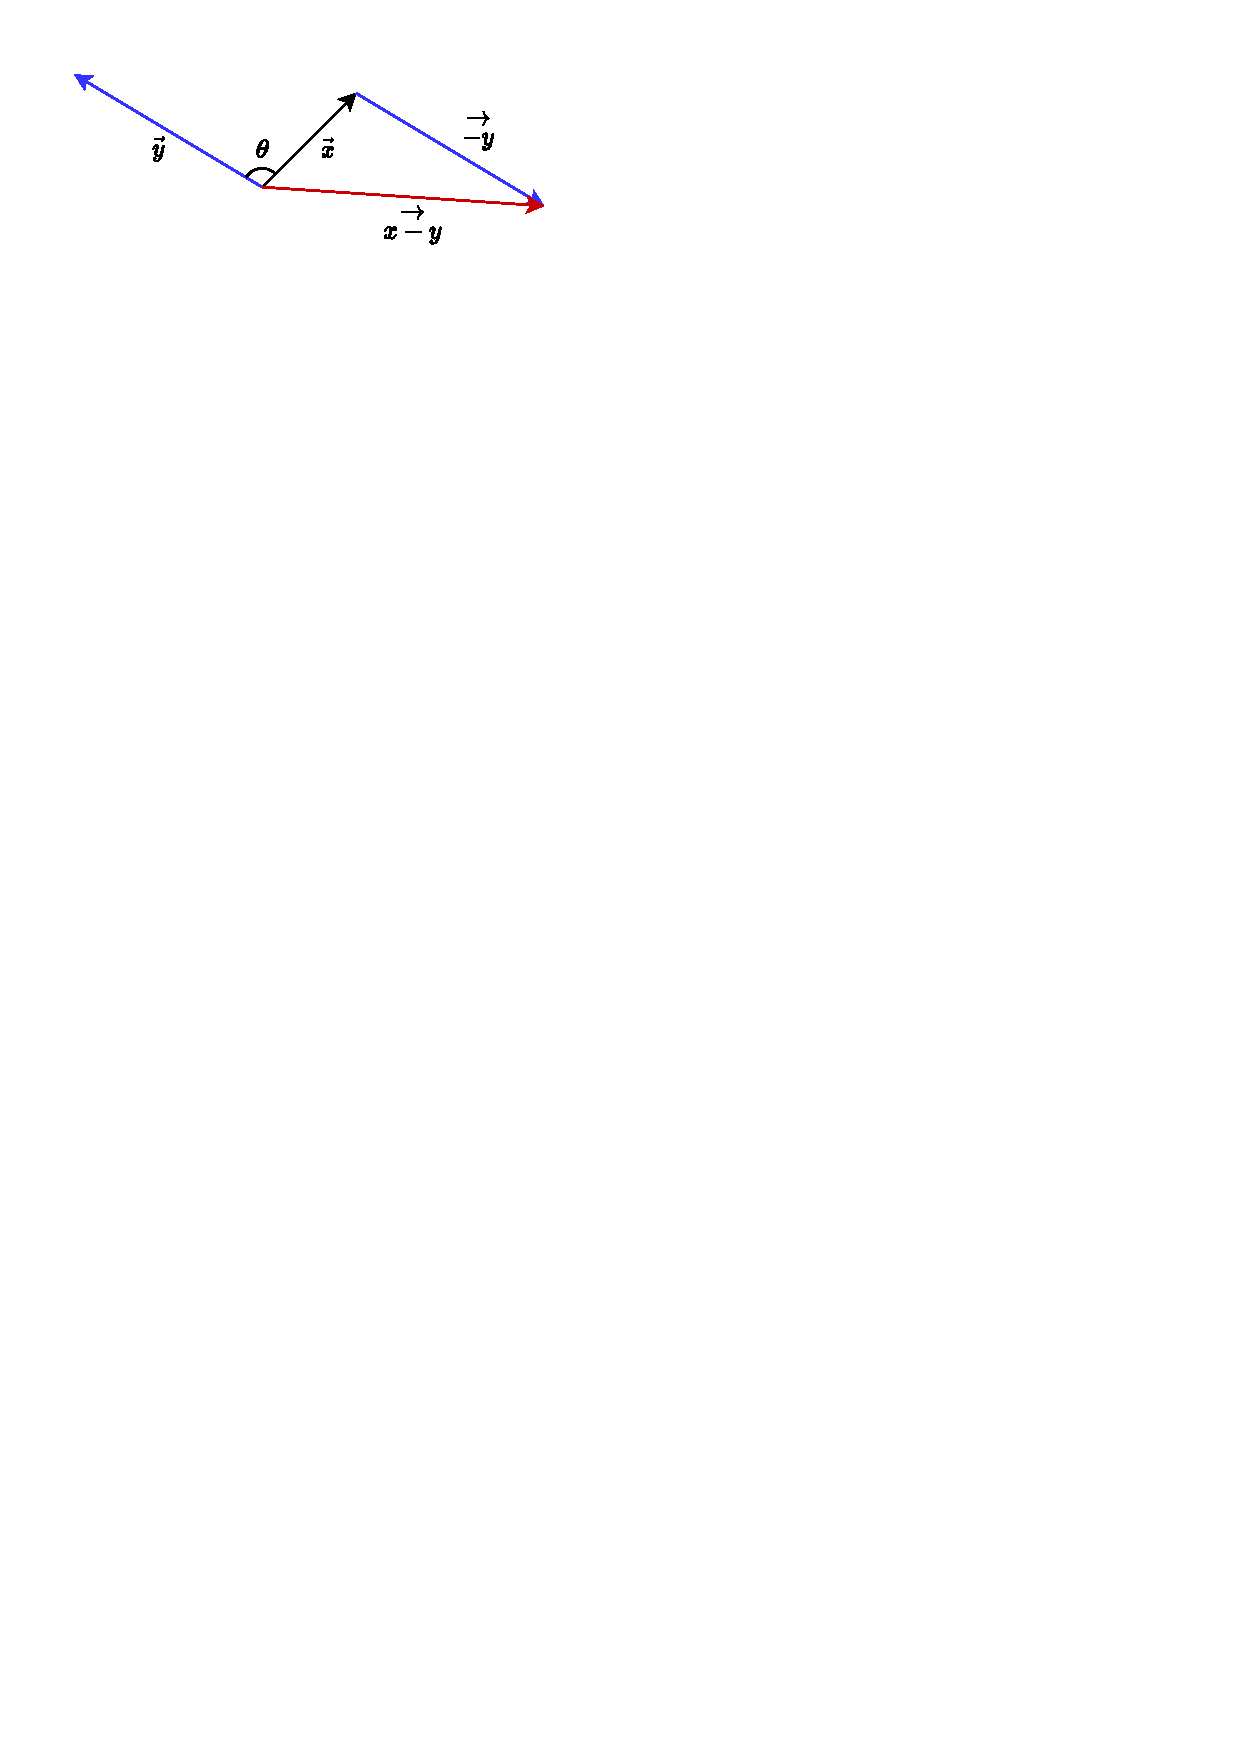
\includegraphics[width=0.4\textwidth]{img/0096.pdf}



证明过程: \\
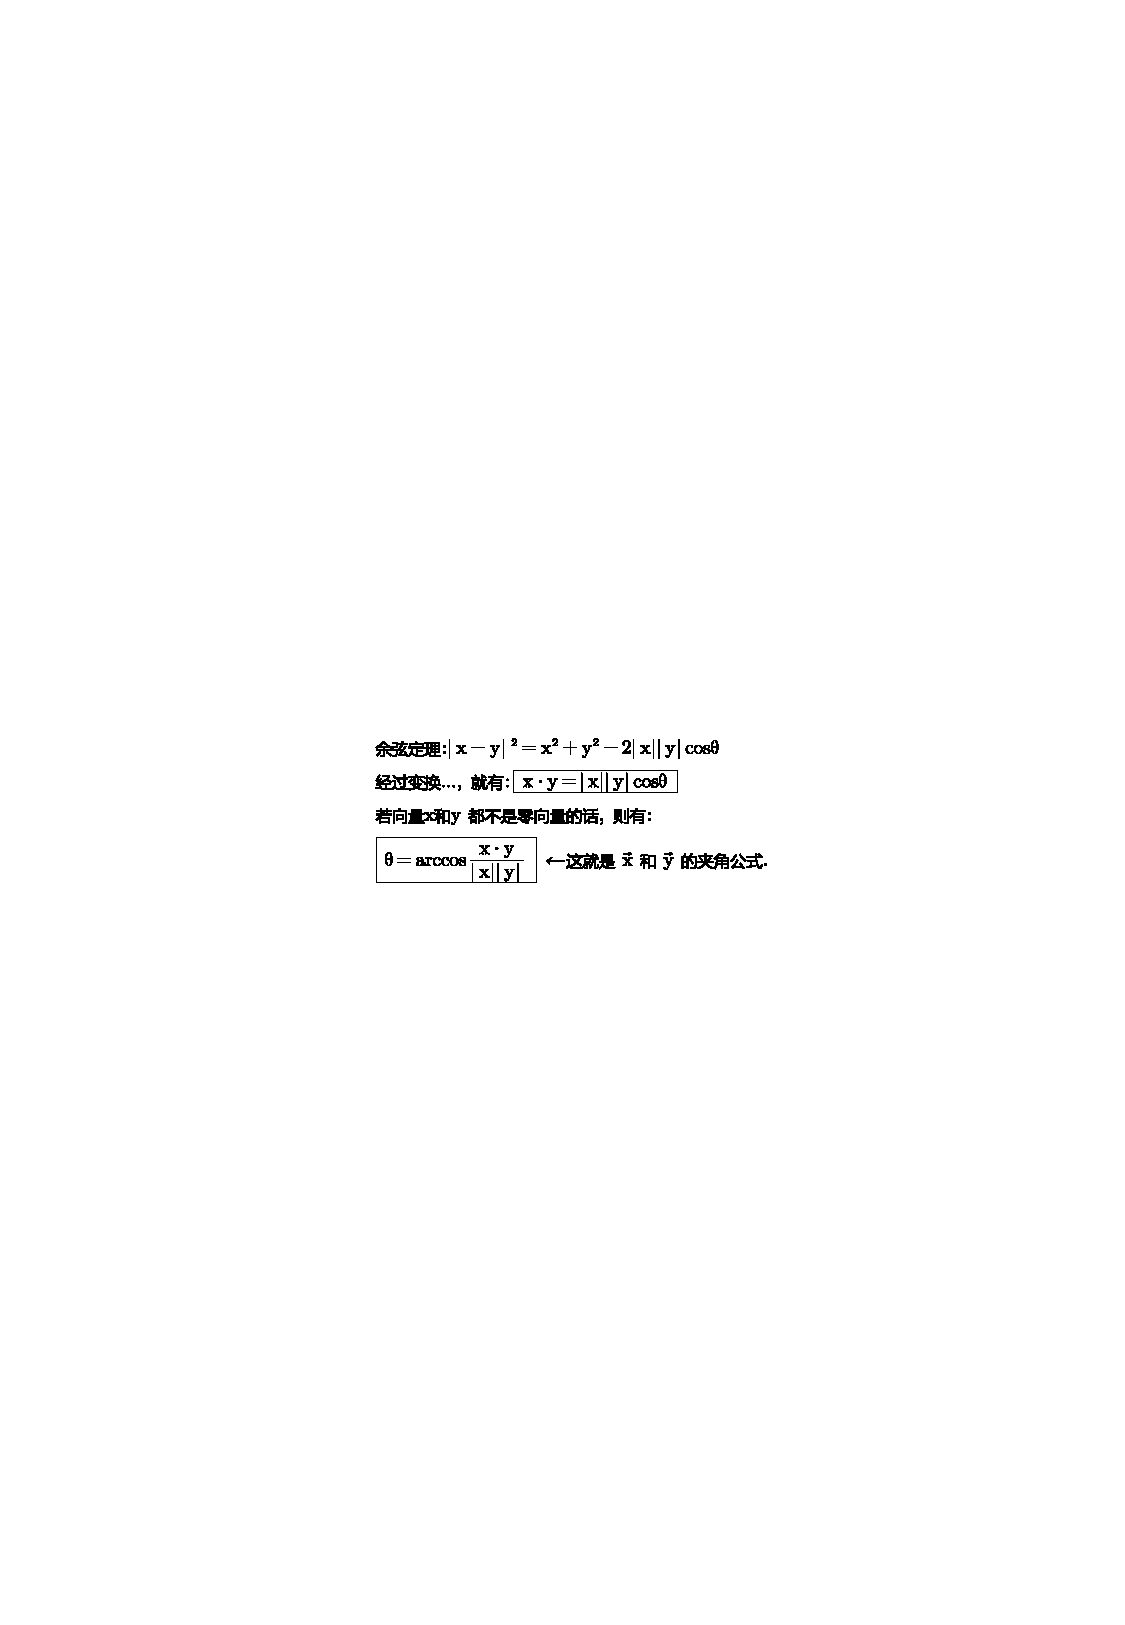
\includegraphics[width=0.55\textwidth]{img/0100.pdf}\\



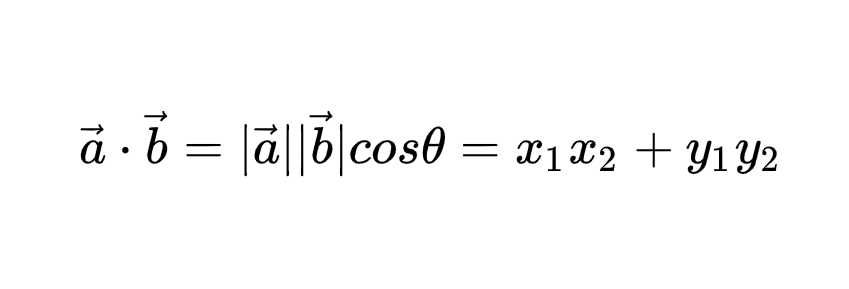
\includegraphics[width=0.4\textwidth]{img/0097.png}
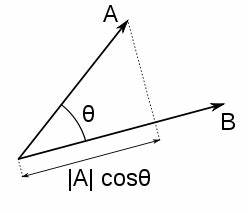
\includegraphics[width=0.2\textwidth]{img/0098.png} \\
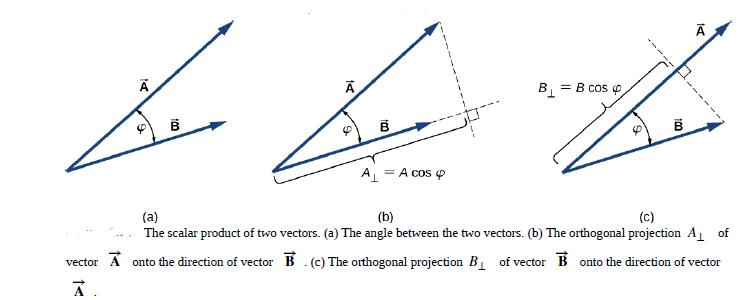
\includegraphics[width=0.9\textwidth]{img/0099.png} \\

根据这个公式, 就可以计算向量a和向量b之间的夹角。从而就可以判断这两个向量是否是同一方向,是否正交(也就是垂直), 等方向关系. 具体对应关系为:\\

~\\
\hrule
~\\





\section{线性组合 linear combination}

\subsection{线性组合 : $\beta =k_1\alpha _1+k_2\alpha _2+...+k_n\alpha _n$ }

【线性组合】: \\
有 $ \beta, \alpha_1, \alpha_2, \alpha_n$, 它们都是n维向量. 若存在 $k_1, k_2, ..., k_n$这些系数(即权重), 能使得 $\beta =k_1\alpha _1+k_2\alpha _2+...+k_n\alpha _n$, 则就称 $\beta$ 是向量组$\alpha_1, \alpha_2, \alpha_n$的一个``线性组合", 或称 $\beta$ 可由向量组$\alpha_1, \alpha_2, \alpha_n$ 来``线性表示". \\

那么这组系数k, 可不可以全取0? 可以. 这样的话,  $\beta=0$ 了. \\


\begin{myEnvSample}
	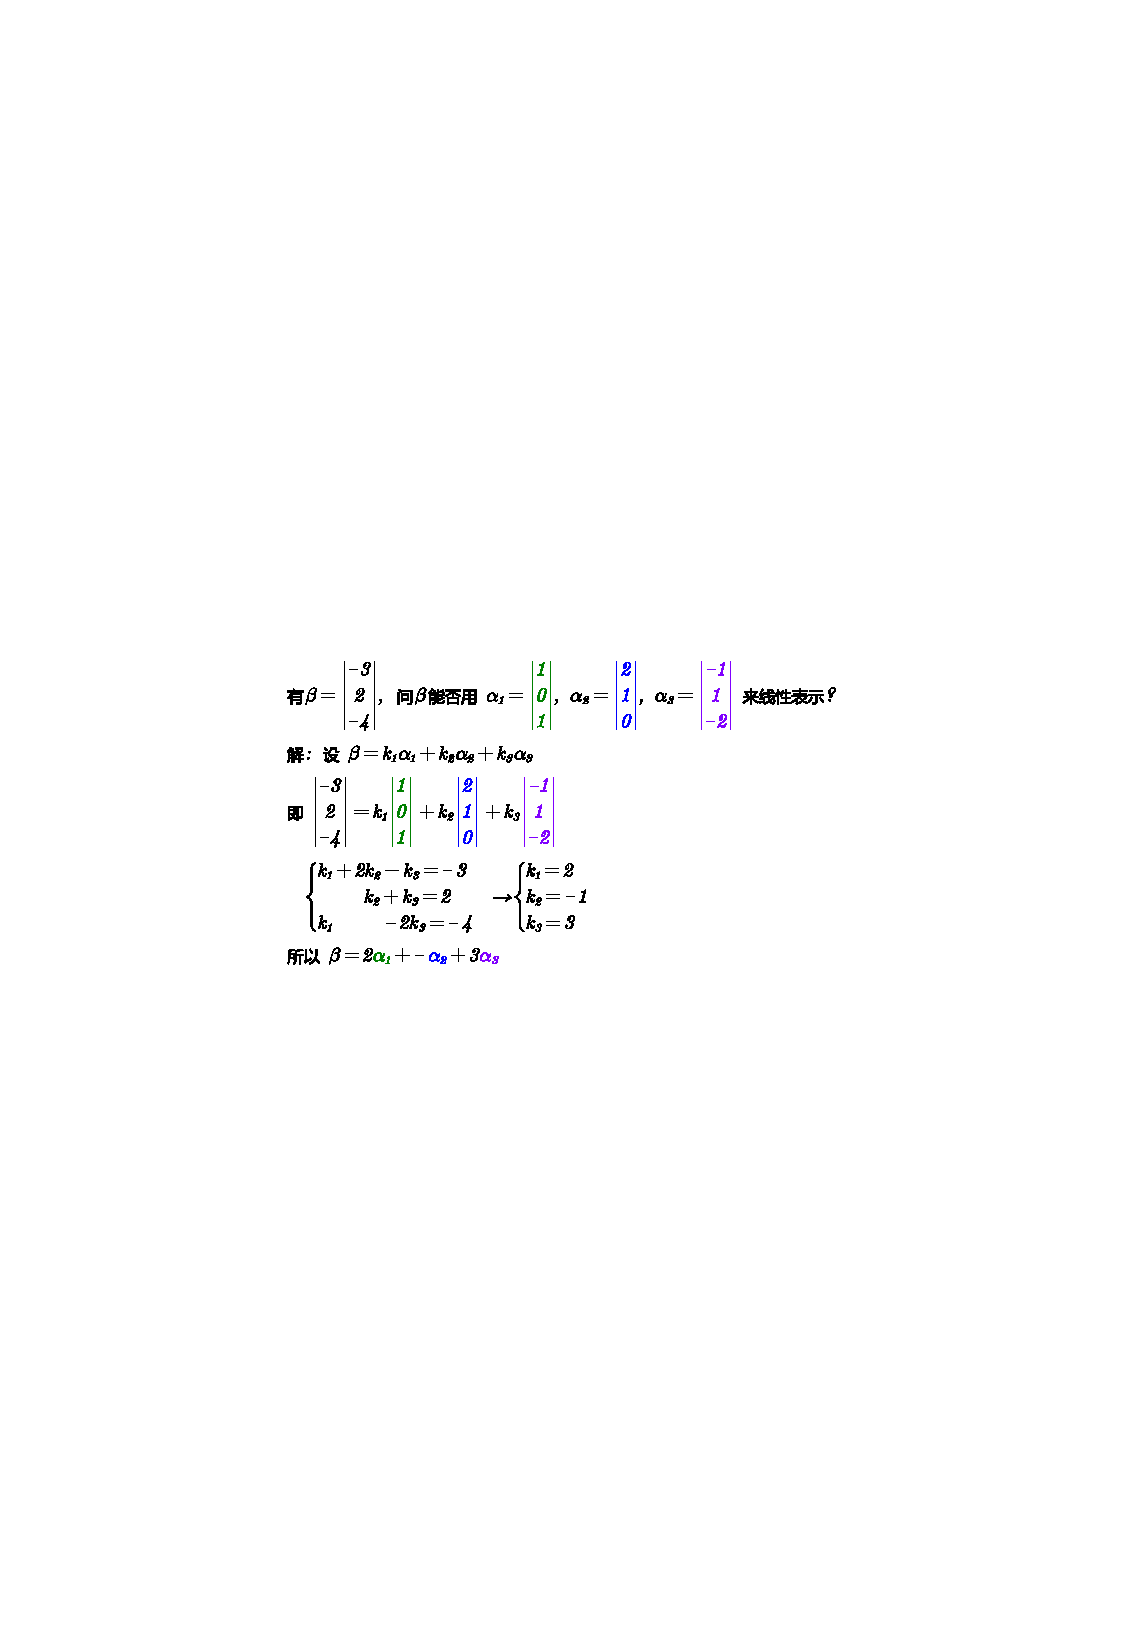
\includegraphics[width=0.75\textwidth]{img/0101.pdf}
\end{myEnvSample}



~\\
\hrule
~\\

\subsection{线性组合的性质}

\subsubsection{性质: 0向量, 可由任意向量组来表示. 即: $0\text{向量}=\ 0\alpha _1+0\alpha _2+...+0\alpha _n$}

~\\
\hrule
~\\

\subsubsection{性质: 向量组A中, 任取出其中的一个向量$α_i$出来, 它可以由这个向量组A来表示. 如: $\alpha _3=0\alpha _1+0\alpha _2+1\alpha _3...+0\alpha _n$}

~\\
\hrule
~\\

\subsubsection{任意一个向量组, 都可由这些个向量(即``n维单位向量")来表示: $\varepsilon _1=\left( 1,0,...,0 \right) ,\ \varepsilon _2=\left( 0,1,...,0 \right) ,\ ...\ ,\varepsilon _n=\left( 0,0,...,1 \right) $}

例如:$
	\left| \begin{array}{c}
		1 \\
		2 \\
		3 \\
	\end{array} \right|=1\left| \begin{array}{c}
		1 \\
		0 \\
		0 \\
	\end{array} \right|+2\left| \begin{array}{c}
		0 \\
		1 \\
		0 \\
	\end{array} \right|+3\left| \begin{array}{c}
		0 \\
		0 \\
		1 \\
	\end{array} \right|
$\\

~\\
\hrule
~\\

\subsection{线性相关}

【线性相关 linearly dependent】: \\
对于n个m维的向量 $ \vec{v_1},  \vec{v_2}, ...  \vec{v_n}$, 若存在一组 k (系数, 倍数)不全为0, 使得 $ k_1  \vec{v_1} + k_2  \vec{v_2} + ... + k_n  \vec{v_n} = 0 $, 则称 $ \vec{v_1},  \vec{v_2}, ...  \vec{v_n}$ 是``线性相关"的.\\

\begin{myEnvSample}
	例如: 下面这三个向量, 是否线性相关?
	\begin{align}
		\left| \begin{array}{l}
			       1 \\
			       0 \\
		       \end{array} \right|,\ \left| \begin{array}{l}
			                                    0 \\
			                                    1 \\
		                                    \end{array} \right|,\ \left| \begin{array}{l}
			                                                                 2 \\
			                                                                 3 \\
		                                                                 \end{array} \right|
	\end{align}

	那么就看下面这个式子, 是否能存在非零的系数 (只要有一个k是不为零的, 就满足了我们的条件)

	\begin{align}
		k_1\left| \begin{array}{l}
			          1 \\
			          0 \\
		          \end{array} \right|+k_2\left| \begin{array}{l}
			                                        0 \\
			                                        1 \\
		                                        \end{array} \right|+k_3\left| \begin{array}{l}
			                                                                      2 \\
			                                                                      3 \\
		                                                                      \end{array} \right|=0
	\end{align}

	那么显然, 当 $ k_1$取2, $k_2$取3, $k_3$取1时, 该式子能成立. 即, 的确存在一组非零的k. \\
	这就说明, 这三个向量, 是``线性相关"的. (不需要所有的系数k都不为0, 只要有一个系数k不为零就行了.)
\end{myEnvSample}


若只能是 k全为0时, 该等式才成立, 那么这些向量 $ \vec{v_1},  \vec{v_2}, ...  \vec{v_n}$ 就是``线性无关"的 (linearly independent). \\

\textbf{``线性无关"就表示, 这组向量中的任何一个, 都无法表示成其他向量的``线性组合". 即, 它们中每一个向量, 都是``独当一面"的, 无法被其他向量所替代.}

~\\
\hrule
~\\

\subsection{线性无关}

不是线性相关, 就是``线性无关"了.

~\\
\hrule
~\\

\subsection{线性相关的 性质, 定理}

\subsubsection{向量组中, 若其中有两个向量成比例, → 则该向量组中的所有成员, 就都``线性相关".}

如:
\begin{align*}
	\underset{ \text{注意:\ 这两个向量成比例}}{\underbrace{(-1)\left| \begin{array}{l}
				                                                                  1 \\
				                                                                  2 \\
			                                                                  \end{array} \right|+(-\frac{1}{2})\left| \begin{array}{l}
				                                                                                                           2 \\
				                                                                                                           3 \\
			                                                                                                           \end{array} \right|}}+0\left| \begin{array}{l}
		                                                                                                                                         5  \\
		                                                                                                                                         19 \\
	                                                                                                                                         \end{array} \right|+0\left| \begin{array}{l}
		                                                                                                                                                                     -1 \\
		                                                                                                                                                                     99 \\
	                                                                                                                                                                     \end{array} \right|=0
\end{align*}

~\\
\hrule
~\\

\subsubsection{含有0向量的任一向量组, 必``线性相关".}

如:
\begin{align*}
	0\vec{v}_1+0\vec{v}_2+0\vec{v}_3+\underset{\text{随便取值}}{\underbrace{k}}\cdot \underset{\text{零向量}}{\underbrace{\vec{0}}}=0
\end{align*}

该向量组, 最后含有一个零向量, 该零向量前的k可以随便取值, 都不影响$k\vec{v}=\vec{0}$. 既然k可以随便取值, 那我们就有了一组不全为0的系数($k_1, k_2, ...k_n$) , 所以这些v向量, 就是``线性相关"的关系了. 

~\\
\hrule
~\\

\subsubsection{只有一个零向量, 则它必``线性相关".}

如:  $k\vec{0}=\vec{0}$ \\
k可以随便取值, 都不妨碍  $ k \cdot \vec{0}= \vec{0}$. 既然k可以随便取值, 那我们就有了一组不全为0的系数( $ k_1, k_2, ...k_n$) , 所以这些v向量(本例中只有一个向量), 就是"线性相关"的关系了.

~\\
\hrule
~\\

\subsubsection{若 $\vec{v_1}, ... \vec{v_r}$ 这组向量是"线性相关"的, 则给它们添加一些新的向量, \\它们整体($\vec{v_1}, ... \vec{v_r}, \vec{v_{r+1}}, ... \vec{v_s}$ ) 依然是"线性相关"的.}

证明过程, 如: \\
已知 $\vec{v_1}, \vec{v_2}, \vec{v_3}$ 是``线性相关"的, 即: \\
$k_1\vec{v}_1+k_2\vec{v}_2+k_3\vec{v}_3=0 $\\

把它扩充一下, 就有:\\
$(k_1\vec{v}_1+k_2\vec{v}_2+k_3\vec{v}_3) +(0\vec{v}_4+0\vec{v}_5)=0$\\

这5个系数k, 就是: $k_1, k_2, k_3, 0, 0$, 不全为0! 说明这组向量 $\vec{v_1}, ... \vec{v_5}$ 是``线性相关"的. 证毕.\\

即: 一个向量组中, 只要其中一部分向量是``线性相关"的, 则就可知道: 整个向量组中的全部向量, 都是``线性相关"的.\\

这里的本质就是: \textbf{比如一个队伍, 有1个女的, n个男的. 它满足``有女"性质. 之后无论往队伍里添加多少人, 它依然满足``有女"性质. 因为这个性质, 在最早的队伍中, 就已经被满足了.}\\


即:\\
部分``线性相关"$\overset{\text{能推导出}}{\rightarrow}$整体``线性相关'' \\
整体``线性相关"$\overset{\text{能推导出}}{\rightarrow}$部分``线性相关'' \\

同样就是说: \textbf{整体``无女"的话, 则其中的子集部分也``无女".}






~\\
\hrule
~\\

\subsection{线性无关的 性质, 定理}


\subsubsection{任意一个非零向量, 必``线性无关".}

如: $k\vec{v}$. 因为 $\vec{v} \ne \vec{0}$, 则只能系数 k=0, 这样本例中, 我们就找不到一组不全为0的k, 那么这一向量必``线性无关".


\subsubsection{}










% https://www.bilibili.com/video/BV1aW411Q7x1?p=22&vd_source=52c6cb2c1143f8e222795afbab2ab1b5
% 5.49




----------------

\part{向量组, 及其线性组合}

\part{向量组的线性相关性}

\part{向量组的秩}

\part{线性方程组的解的结构}

\part{向量空间}



\end{document}